\pagenumbering{arabic} %necessary to start numbering pages in arabic numerals from here
\setcounter{page}{1} 

\section{Introduction}  
Breast cancer is a highly heterogeneous disease, meaning that there is a high degree of genotypic and phenotypic diversity within and between tumours, with much of this heterogeneity being attributed to the high frequency of mutations within the genome, also referred to as genomic instability (GI) \citep{pmid31078431, pmid36624542}. Breast cancer classification and selection of treatment regimen are currently based on clinical and histopathological features \citep{pmid23395906, pmid36482272}, with recent research focused on utilising markers derived from genomics data to expand our understanding of the molecular mechanisms underlying breast cancer and to improve patient outcome by identifying patients who may not be well classified by the standard tissue-based biomarkers \citep{pmid22522925, pmid23395906, pmid31413819, pmid37564937}.   
 
Copy number variations (CNVs) and copy number alterations (CNAs), forms of GI, are changes in the copy number of a DNA sequence in the form of either a gain or loss, occurring in germline and somatic cells, respectively \citep{pmid19566914, pmid23412801, pmid31874603}. In the context of cancer, focus is primarily given to CNAs, their potential to initiate cancer through activation of oncogenes and inactivation of tumour suppressor genes, and their associations with disease progression and survival \citep{pmid20033038, pmid27161491, pmid30178746, pmid30526857, pmid31085648, pmid36806386}.  

The aim of this thesis is to assess whether CNA information, in isolation or in combination with clinical and gene expression data, improves predictive models of overall survival (OS) and disease-specific survival (DSS) for breast cancer patients. We explore this by proposing several novel CNA metrics that quantify the levels of CNAs across the whole genome and across chromosome arms and assess the role the distribution of these metrics have in the context of OS and DSS. We go further, examining the role of the allele-specific CNA landscape, exploring statistical models to detect and model features of changepoints in allele-specific CNA profiles. 

\subsection{Breast Cancer in the Clinical and Research Setting}  
Breast cancer is one of the most common malignancies affecting women worldwide and is one of the leading causes of cancer related death among this group \citep{pmid28223433, pmid33538338}. Cancer that develops in breast cells typically forms in either the lobules (lobular carcinoma) or the milk ducts (ductal carcinoma). Cancer cells that remain in the milk ducts or lobules and do not grow into or invade normal tissues within or beyond the breast are termed non-invasive, also sometimes called carcinoma in situ (“in the same place”) or pre-cancers. Invasive breast cancer, where there is spread of cancer cells outside of the ducts and lobules into the surrounding normal tissue, is most commonly observed in breast cancer patients \citep{pmid24716497, pmid28969709}.    

Tests used to diagnose breast cancer include mammograms, ultrasounds and biopsies \citep{pmid19930975}. Breast cancer classification and treatment generally follows an integrative approach whereby both clinical information and tissue-based biomarkers are used \citep{pmid23395906, pmid28733194}. These clinical and histopathological features include age, histological grade, tumour size, nodal status, oestrogen receptor (ER), progesterone receptor (PR) and human epidermal growth factor receptor 2 (HER2) status, amongst others \citep{pmid28733194, pmid36482272}. Current classification of breast cancer in the clinical setting is based on immunohistochemical staining determining ER, PR and HER2 status, with measurement of ER, PR and HER2 being mandatory in all newly diagnosed breast cancer cases \citep{pmid28882552}. Based on hormone receptors (HR), i.e. combinations of ER and PR, and HER2 positivity, patients are classified as HR+/HER2-, HR-/HER2-, HR+/HER2+ or HR-/HER2+ \citep{pmid20520800}.   

In published research, gene expression and CNA data have been used to produce molecular classifications of breast cancer along with a number of prognostic and predictive assays, providing information about likely survival outcome and response to therapy \citep{pmid10963602, pmid22522925, pmid28882552}. Molecular-based classifications, being evaluated in the research setting, but not yet common place in routine clinical use, include the Prediction Analysis of Microarray 50 (PAM50) intrinsic subtypes and Integrative Clusters (IntClust) \citep{pmid10963602, pmid12829800, pmid22522925}. PAM50 is a 50-gene signature that classifies breast cancer into five molecular intrinsic subtypes, Luminal A, Luminal B, HER2-enriched, Basal-like and Normal-like, that have been shown to have both prognostic and predictive power. Briefly, using complementary DNA (cDNA) microarrays on 65 breast cancer samples \cite{pmid10963602} identified a subset of 496 genes whose variation in expression was significantly greater between samples from different tumours than between samples from the same tumour. Performing hierarchical clustering with this “intrinsic” gene subset resulted in the samples being split into four groupings related to different biological features (ER+/Luminal-like, Basal-like, HER2-enriched and Normal-like). Subsequently, using the same intrinsic gene set, \cite{pmid11553815} performed hierarchical clustering on 85 breast tumour cDNA microarrays. In addition to classifying samples into Luminal-like, Basal-like, HER2-enriched and Normal-like groups, the Luminal-like group was further divided into at least two subgroups, each with a distinctive gene expression profile. \cite{parker} later developed the 50-gene subtype predictor (PAM50) by performing gene set reduction on the 496 intrinsic genes \citep{pmid10963602, pmid11553815}, along with an additional 1,410 identified in three other microarray studies \citep{micro1, micro2, micro3}. Claudin-low, a sixth subtype of breast cancer identified using gene expression data in a separate study \citep{pmid17493263, pmid20813035}, is also considered an intrinsic subtype \citep{pmid32286297}. \cite{TCGA}, integrating DNA copy number arrays, DNA methylation, exome sequencing, messenger RNA arrays, microRNA sequencing and reverse-phase protein arrays, also observed the existence of four main breast cancer classes, each of which shows significant molecular heterogeneity in terms genetic and epigenetic alterations and are highly correlated with PAM50 subtype. IntClust derived from gene expression and CNA data classifies breast cancer into ten integrative clusters, IntClust 1-10, each with distinct CNA landscape, risk patterns and prognosis \citep{pmid22522925}. Prognostic biomarkers include ER, PR, HER2 and Ki67 status, Urokinase plasminogen activator/plasminogen activator inhibitor 1 (uPA/PAI-1), Oncotype DX, MammaPrint, Prosigna and Breast Cancer Index (BCI), while predictive biomarkers include ER status, PR status, HER2 status, deficiency in DNA damage response (DDR), mutational status of ER, amongst others \citep{pmid24402422, pmid28882552}. 

\subsection{Molecular Taxonomy of Breast Cancer International Consortium Data} 
The data used in this thesis are from the Molecular Taxonomy of Breast Cancer International Consortium (METABRIC) study \citep{pmid22522925}. The datasets, collected from five centres in the United Kingdom and Canada between 1977-2005, are well-annotated and contain clinical, transcriptomic and genomic data for approximately 2,000 breast cancer cases. The processed METABRIC datasets are publicly available from cBioPortal (http://www.cbioportal.org/study?id=brca\_metabric) \citep{pmid22588877, pmid23550210}. For the focus of this thesis, only the clinical, transcriptomic and CNA data are used.   

The clinical data includes information on approximately 25 variables including age at diagnosis, Nottingham Prognostic Index (NPI), number of lymph nodes positive, tumour size, ER, PR and HER2 status, tumour stage, histological grade, PAM50 subtype (with Claudin-low) and IntClust classification, where IntClust 4 is split into IntClust 4ER+ and 4ER-, resulting in 11 IntClusts (Table \ref{Clinchar}). Figure \ref{fig:Comp} displays the distribution of PAM50 subtypes within each IntClust. Available treatments to this cohort of patients were hormone therapy, chemotherapy, radiotherapy and breast surgery, as summarised in Table \ref{Treatment}. Enrolment of patients into the METABRIC study predated availability of trastuzumab (Herceptin). The survival outcomes recorded are OS, defined as the time from breast cancer diagnosis to death from any cause, DSS, defined as the time from breast cancer diagnosis to death from cancer, and recurrence-free survival (RFS), defined as the time from breast cancer diagnosis to relapse (Table \ref{SurvTable}). From the OS and DSS variables, 5- and 10-year OS and DSS are generated for each patient, e.g. if a patient experienced an event at 5 years and 1 month (61 months), then they would be censored (0) at 5 years (60 months). While most clinical variables are recorded for a large proportion of patients, some missingness exists.    

Copy number for tumours observed in the METABRIC cohort were measured with the Affymetrix single-nucleotide polymorphism (SNP) 6.0 array, with pre-processing and quality control steps implemented by \cite{pmid22522925} to obtain $\text{log}_2$ intensity values. For each tumour sample, the $\text{log}_2$ ratio (the ratio between the observed $\text{log}_2$ intensity value and the expected $\text{log}_2$ intensity value) for each probe was calculated by subtracting a “normal” pooled reference, generated using the HapMap \citep{pmid14685227} and matched normal datasets, from the tumour sample $\text{log}_2$ intensities. After computing the $\text{log}_2$ ratios for each probe, \cite{pmid22522925} applied the circular binary segmentation (CBS) algorithm \citep{pmid15475419, pmid17234643}, using DNAcopy \citep{DNAcopy}, to each sample to detect changepoints and divide the genome into regions of equal copy number. CNAs were then called using selected thresholds for gains and losses across the whole genome, and genes affected by CNAs identified by gene annotation using hg18 \citep{pmid22522925}. The summary CNA data contains patient-specific somatic CNA calls for each of the 22,544 annotated genes and has values indicating homozygous deletion (-2), hemizygous deletion (-1), diploidy (0), single copy gain (+1) and high-level amplification (+2).  
 
The transcriptomic data include $\text{log}_2$ transformed and normalised gene expression and z-score data, measured with the Illumina HT-12v3 array. The log intensity z-score data contain information on the number of standard deviations away a gene's expression is from its mean expression across all profiled samples. This measure is useful to determine whether a gene in one patient's tumour sample is up or down-regulated relative to all other tumour samples.   

\vfill 
\begin{table}[!h]
\caption{Selected clinical characteristics of the METABRIC patients.}
\begin{minipage}[c]{0.5\textwidth}
\centering
\begin{tabular}{ccc}
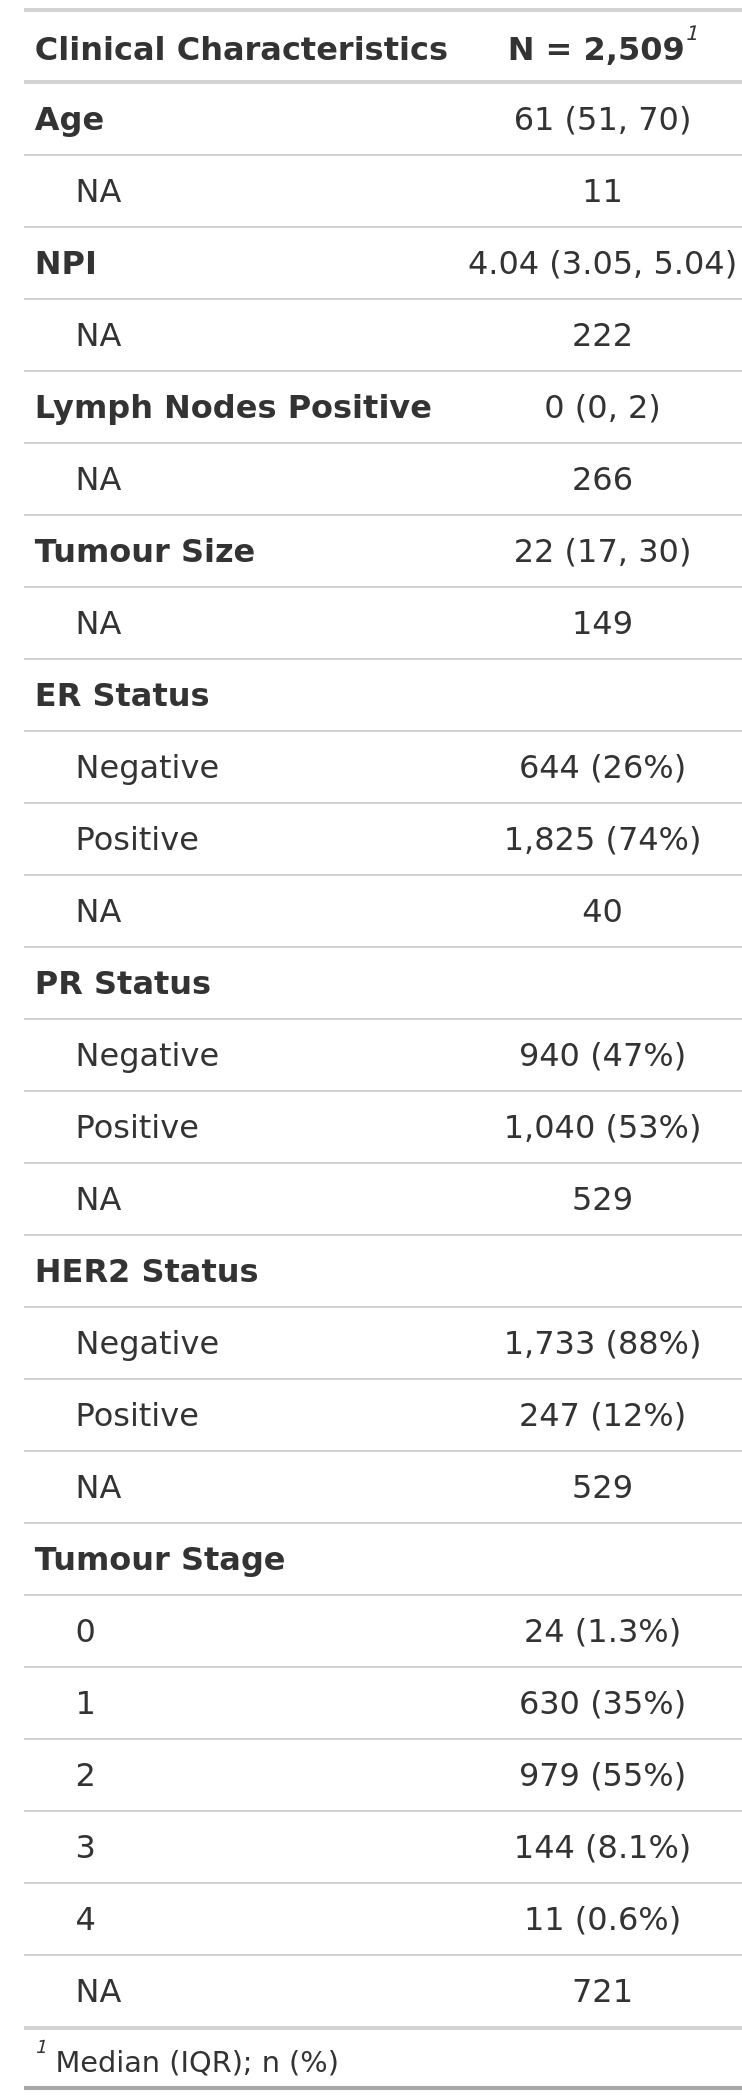
\includegraphics[height = 18cm]{../tables/Introduction/Table1_Clin_pt1.png}
\end{tabular}
\end{minipage}
\begin{minipage}[c]{0.5\textwidth}
\centering
\begin{tabular}{ccc}
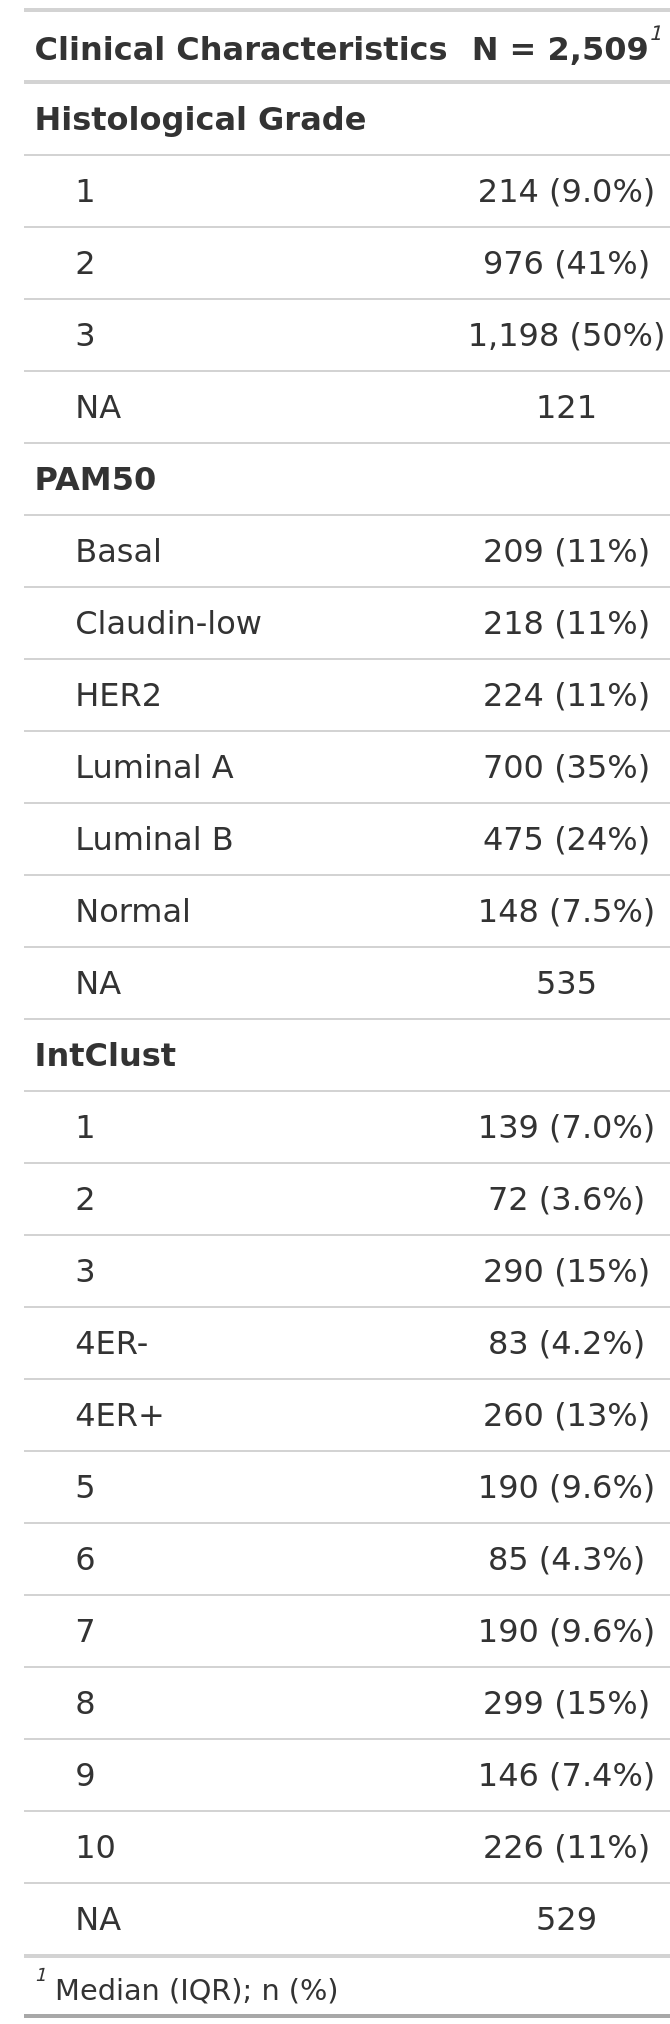
\includegraphics[height = 18cm]{../tables/Introduction/Table1_Clin_pt2.png}
\end{tabular}
\end{minipage}
\label{Clinchar}
\end{table}
\vfill 
\clearpage

\begin{figure}[H]
\center
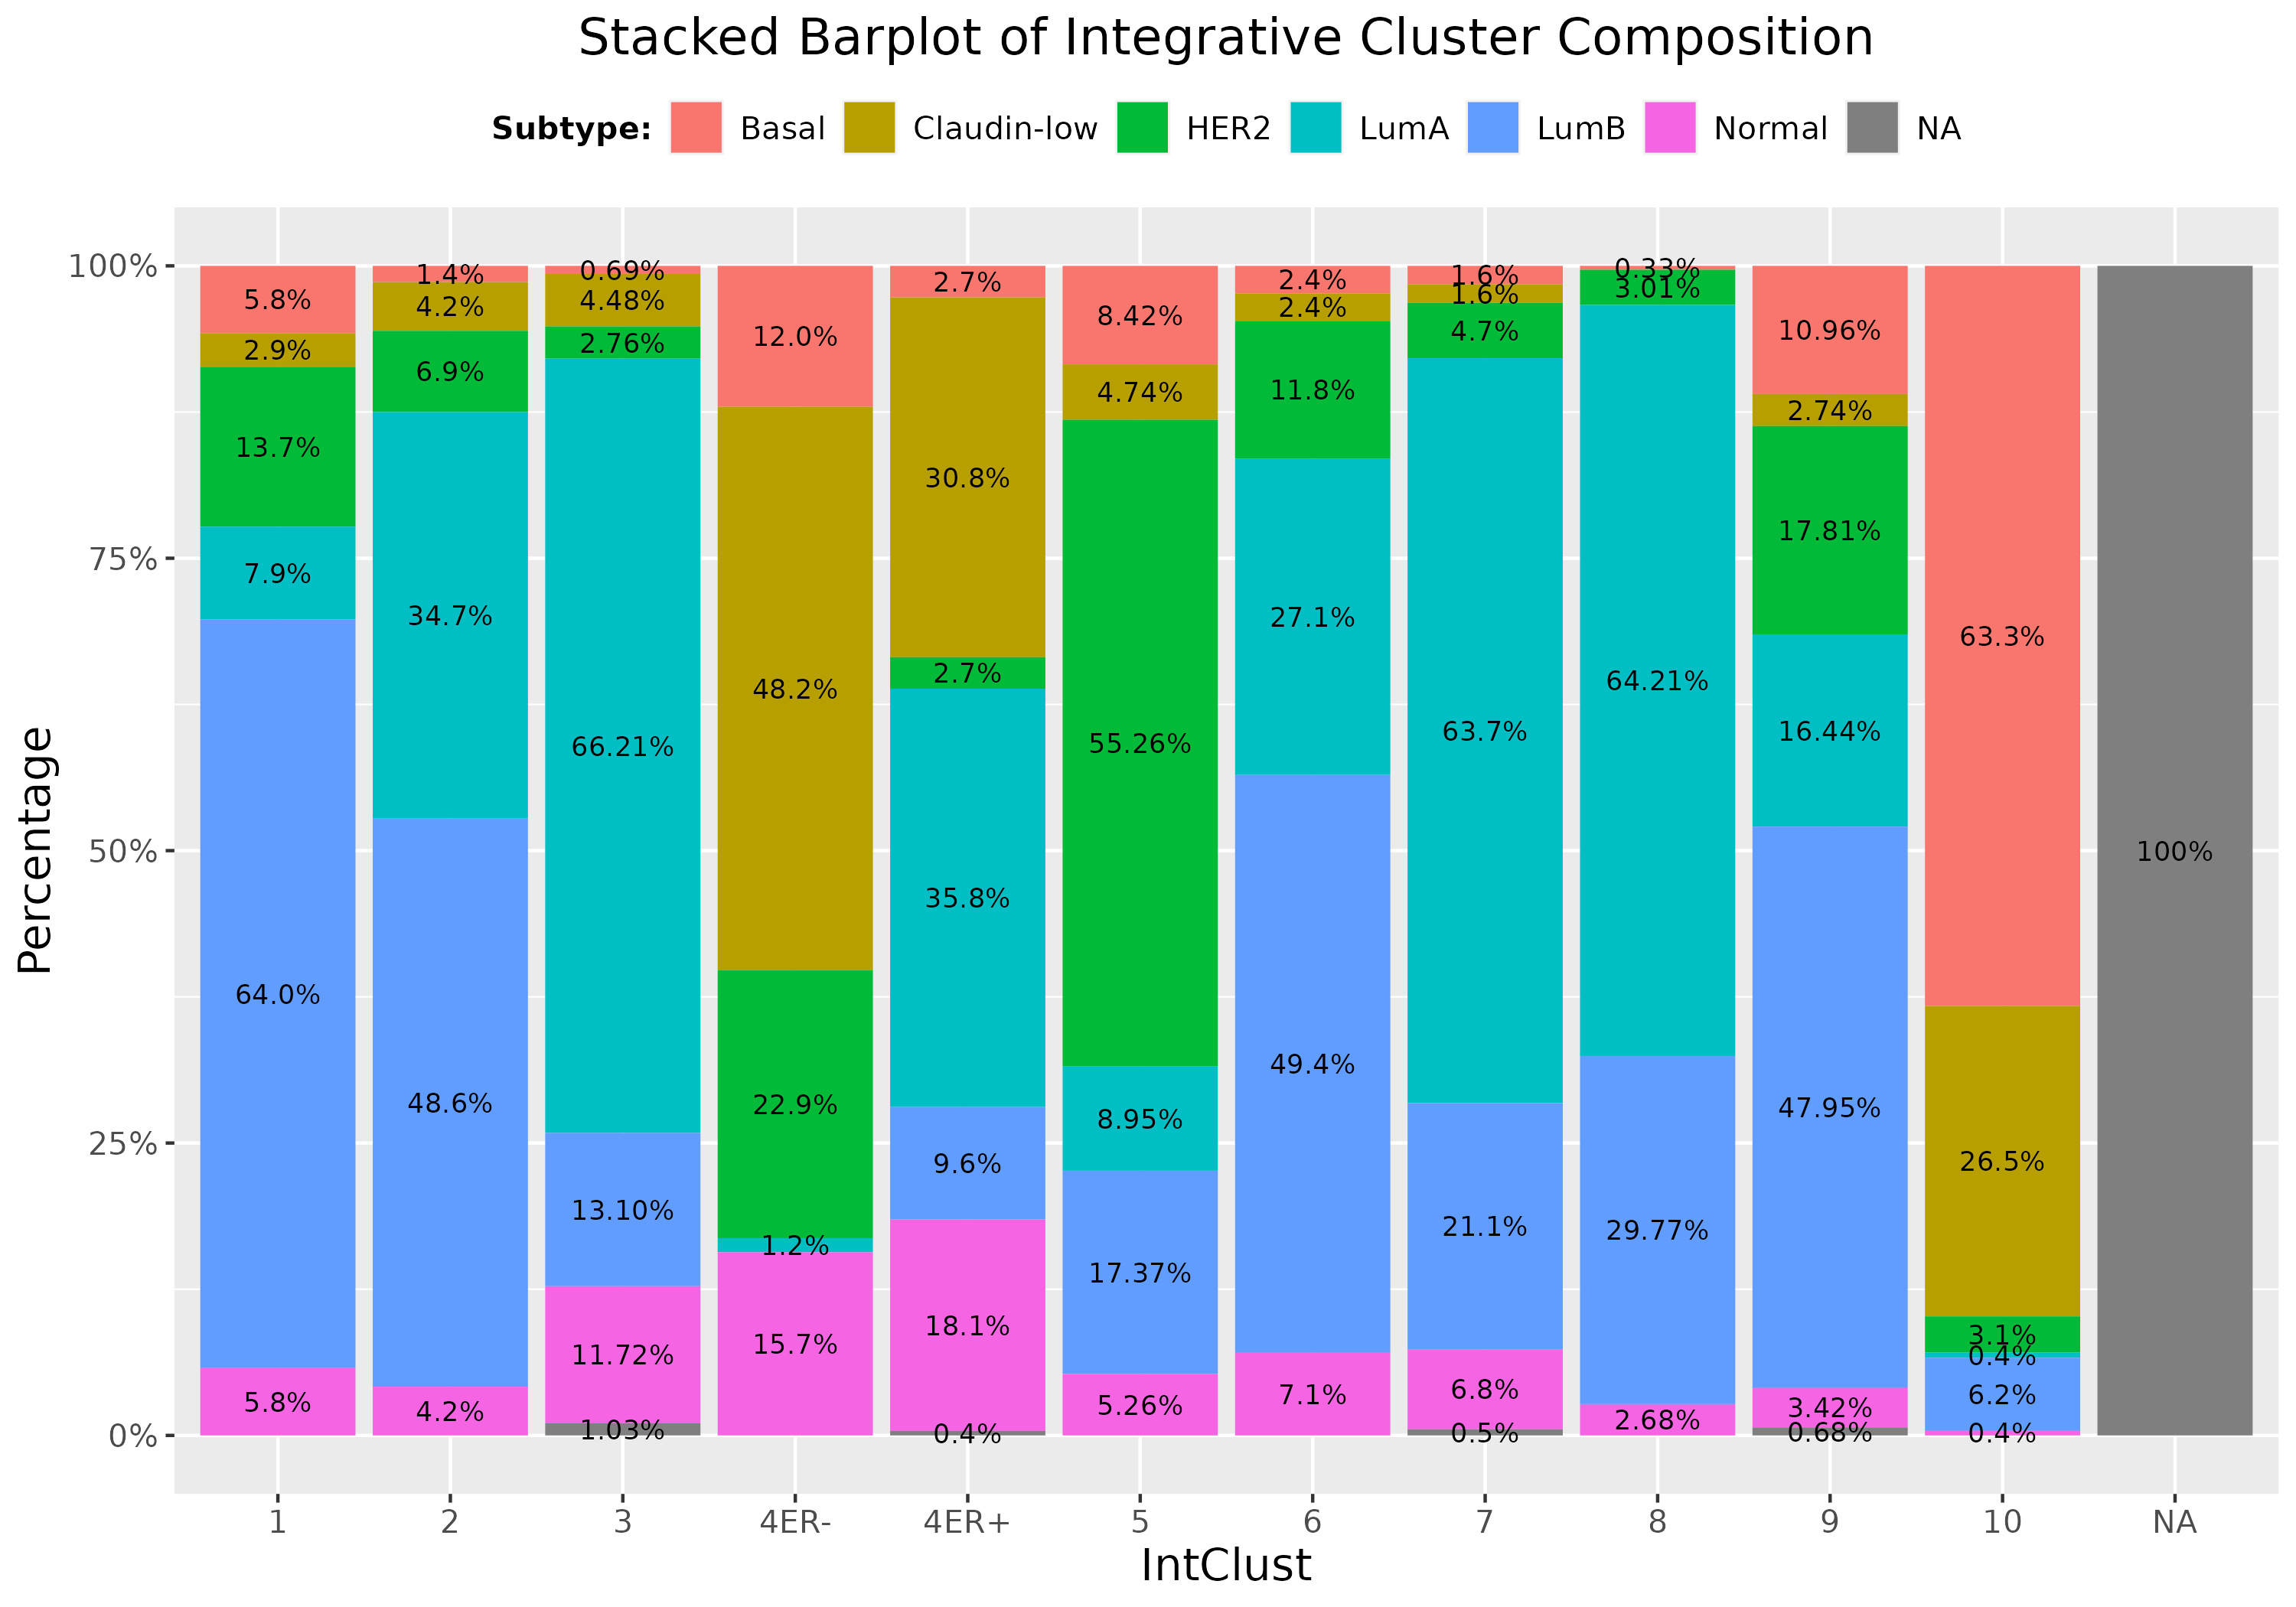
\includegraphics[width=0.94\textwidth]{../figures/Introduction/IntClust_Composition.png}
\caption[Stacked barplot indicating the PAM50 composition of each Integrative Cluster.]{Stacked barplot indicating the PAM50 composition of each Integrative Cluster. The x-axis denotes the Integrative Clusters and the y-axis percentages.}
\label{fig:Comp}
\end{figure} 

\begin{table}[H]
%\hspace{-1cm}
\begin{minipage}[c]{0.48\textwidth}
\centering
\caption{Treatment characteristics of the METABRIC patients.}
\begin{tabular}{ccc}
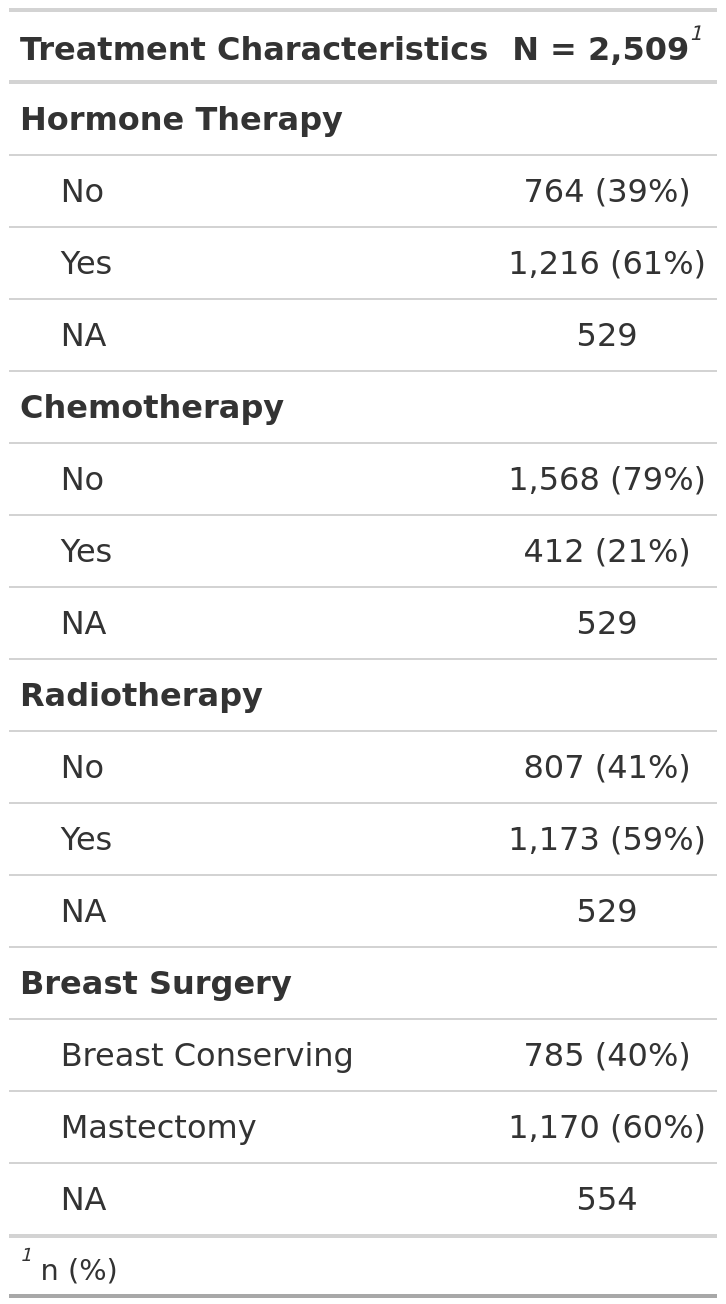
\includegraphics[height = 10.8cm]{../tables/Introduction/Table2_Treatment.png}
\label{Treatment}
\end{tabular}
\end{minipage}
\hspace{0.4cm}
\begin{minipage}[c]{0.48\textwidth}
\centering
\caption{Survival characteristics of the METABRIC patients.}
\begin{tabular}{ccc}
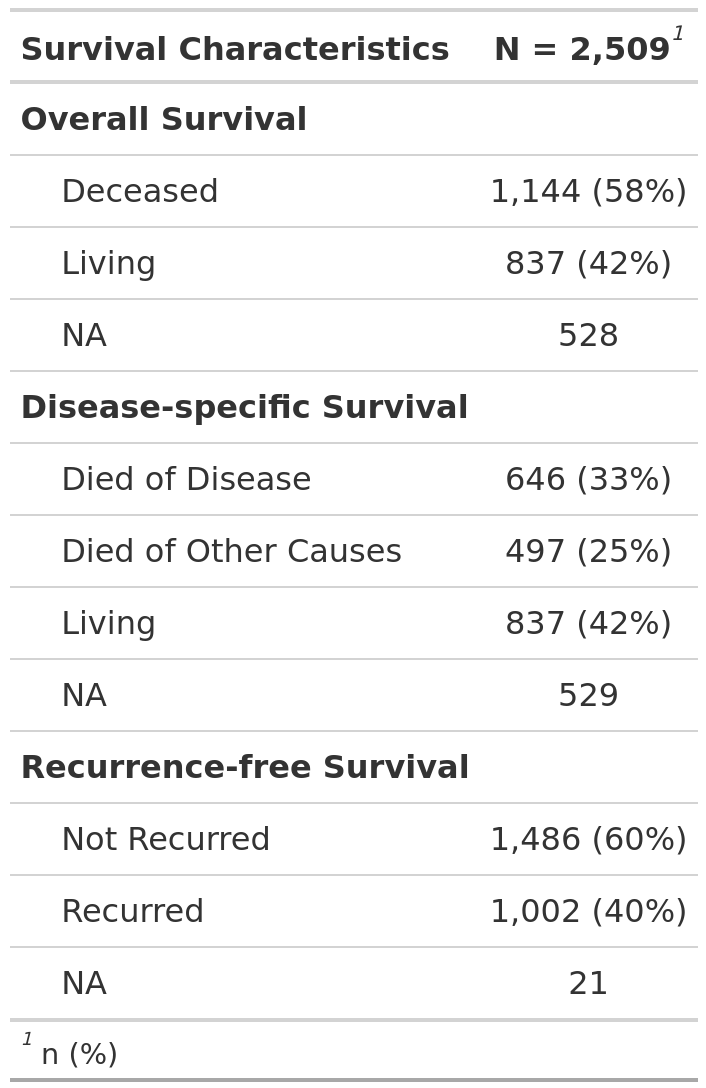
\includegraphics[height = 10.8cm]{../tables/Introduction/Table3_Survival.png}
\label{SurvTable}
\end{tabular}
\end{minipage}
\end{table}
 
These publicly available data are highly curated and periodically updated with additional information or datasets. Throughout this thesis the processed METABRIC data downloaded from cBioPortal are used “as is” and with the training and test sets defined in \cite{pmid22522925}, combined. Unless otherwise stated the results discussed in this thesis are based on the processed METABRIC data downloaded from cBioPortal in 2021.   

To obtain allele-specific CNA profiles, 1,992 Affymetrix SNP 6.0 CEL files available for 1,992 patients in the METABRIC study were accessed from the European Genome Phenome archive (study accession EGAS00000000083) \citep{pmid22522925, pmid34791407}. 

\subsection{Structure of Thesis}
Chapter 2 discusses CNAs as a measure of GI, with an introduction to published approaches for quantifying GI, and GI patterns in breast cancer. With application to the METABRIC cohort, novel CNA metrics are proposed, to measure individual patient CNA burden, accounting for the type, magnitude and location of the CNA. The distributions of the CNA metrics observed for the cohort are summarised, with an assessment of any effect from missing values. Distributions of CNA metrics are produced and summarised given location, e.g. global, or chromosome-arm specific, and are analysed comparing patients grouped by pre-defined breast cancer molecular classifications, such as PAM50 and IntClust.  

Chapter 3 investigates whether there is an association between the CNA metrics and survival outcomes, within the METABRIC cohort. A number of parametric, semi-parametric and non-parametric survival models are applied. Applications of survival trees demonstrate splits of patients into classification nodes using the molecular classifications and clinicopathological variables, while introducing the proposed CNA metrics as candidate predictors. 

Chapter 4 examines the effect of CNAs on gene expression, initially describing differential gene expression using limma and several expression-based predictive and prognostic assays for breast cancer. Differential gene expression analysis is carried out comparing gene expression between stratified groups of patients shown to have different survival outcomes, informed by models incorporating the CNA metric information. To finish, a comparative study is conducted, to compare the listing of differently expressed genes arrived at in this thesis, having incorporated CNA metric information, to the listings of prognostic and predictive gene sets previously derived and in use.

Chapter 5 focuses on allele-specific CNA profiles, CNA changepoints, and their identification and classification. The chapter reviews allele-specific copy number profiling using Allele-Specific Copy number Analysis of Tumours (ASCAT). Extraction of allele-specific CNA profiles using the PennCNV and ASCAT software is discussed and applied to the METABRIC cohort. Approaches to identify and model features of changepoints in allele-specific CNA profiles are proposed and include an extensive simulation study. 

Chapter 6 details application of allele-specific models to the METABRIC data. The models are applied to defined intervals, corresponding to gene regions and whole genome segments, and the genes and segments identified as containing CNA changepoints of significant length examined in the context of survival.  